\documentclass[dvipdfmx,aspectratio=169]{beamer}
\usepackage{pxjahyper}							%しおりの文字化けを防ぐ
\renewcommand{\kanjifamilydefault}{\gtdefault}	%日本語フォントをゴシックに
\usepackage{graphics}							%各種画像の張り込み
\usepackage{amsmath,amssymb,mathtools}					%標準数式表現を拡大する
\usepackage{ulem}
\usepackage{ascmac,fancybox}
\usetheme[
	block=fill,
	progressbar=foot,
	numbering=fraction,
	subsectionpage=progressbar
]{Metropolis}
\usefonttheme{professionalfonts}

\usepackage{here}
\usepackage{booktabs}

\usepackage{tikz}
\usetikzlibrary{positioning}
\usepackage{color}

\newcommand{\highlight}[2][yellow]{\tikz[baseline=(x.base)]{\node[rectangle,rounded corners,fill=#1!10](x){#2};}}
\newcommand{\highlightcap}[3][yellow]{\tikz[baseline=(x.base)]{\node[rectangle,rounded corners,fill=#1!10](x){#2} node[below of=x, color=#1]{#3};}}

\title{ディープラーニングの仕組みを知ろう!}
\subtitle{第2回 人工知能勉強会}
\author{Shion MORISHITA}
\institute{}
\date{\today}

\subject{\LaTeX{}+Beamer}
\begin{document}
	%タイトル
	\begin{frame}[plain]
	    \maketitle
	\end{frame}
		
	\begin{frame}[shrink]{目次}
		\vspace{1em}
		\tableofcontents
	\end{frame}
	
	\section{はじめに}
	\begin{frame}{目的}
		\begin{itemize}
			\item
		\end{itemize}
	\end{frame}

	\section{勾配降下法}
	\subsection{勾配降下法の基本概念}
	\begin{frame}{勾配降下法とその目的}
		\begin{itemize}
			\item 機械学習や最適化の分野で広く用いられる最適化アルゴリズム
			\item 目的:最小化(または最大化)したい関数の最適なパラメータを見つけること
		\end{itemize}
		% TODO: \usepackage{graphicx} required
		\begin{figure}
			\centering
			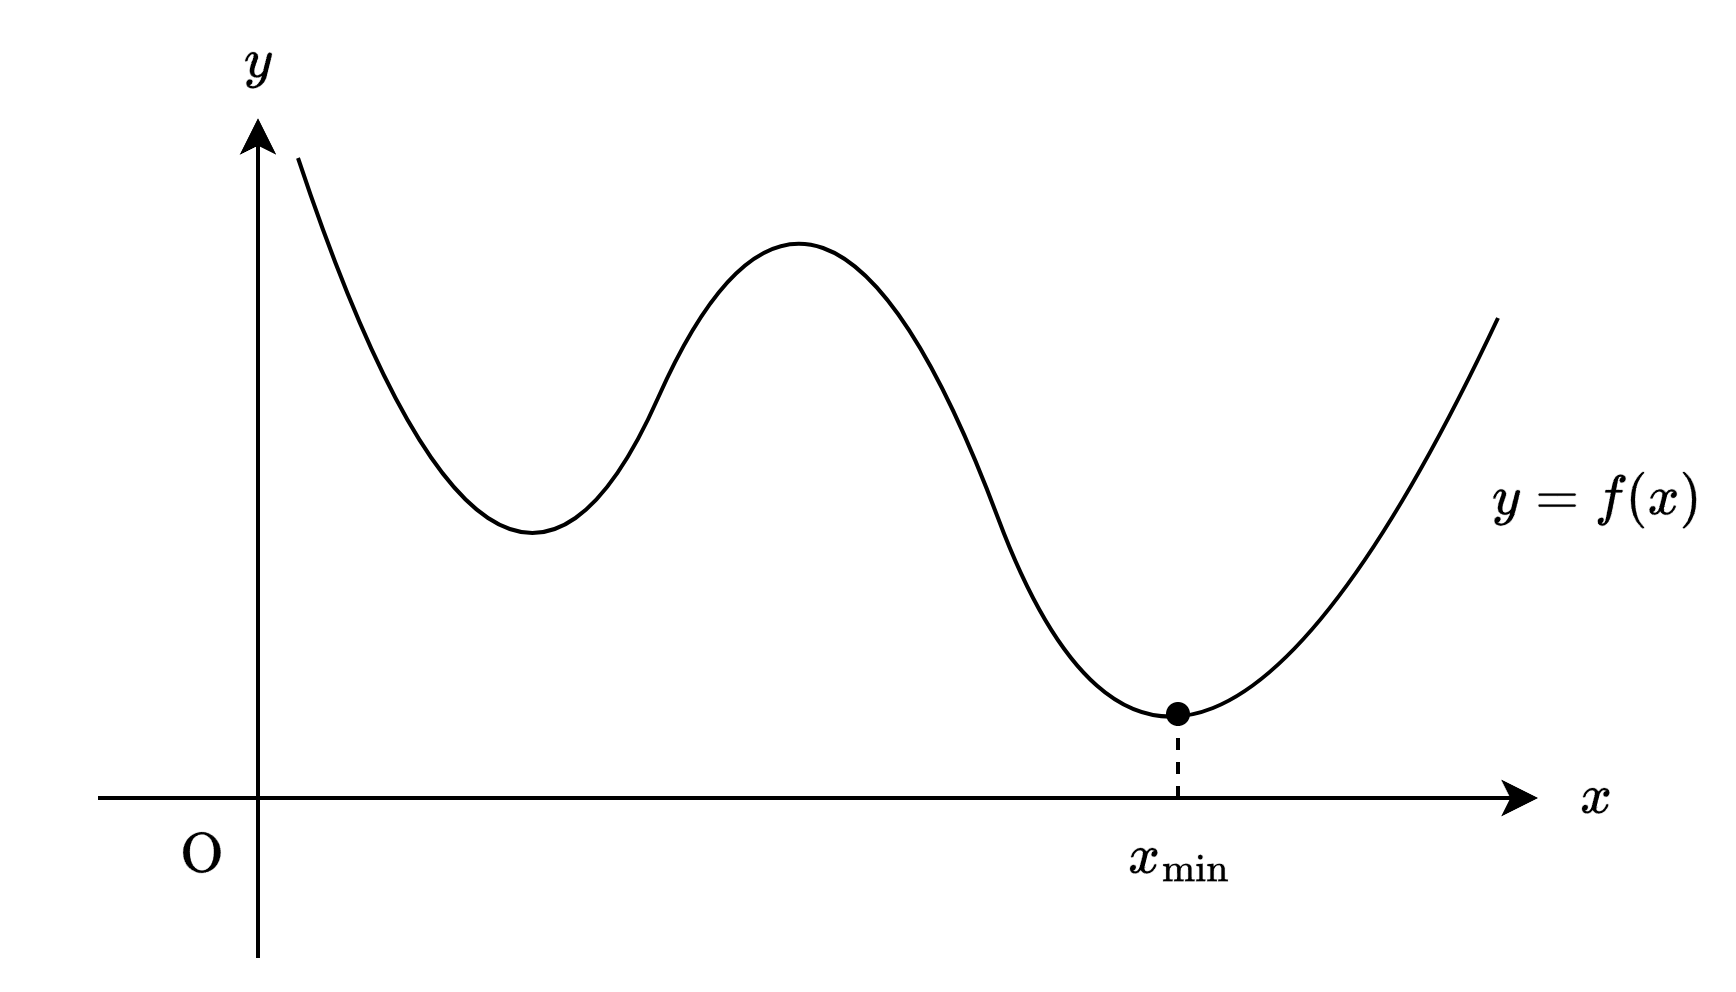
\includegraphics[width=0.65\linewidth]{img/gradient-descent-method-the-point-at-which-the-function-is-minimized}
		\end{figure}
	\end{frame}
	\begin{frame}{勾配降下法のアイデア}
		どのように関数が最小となるパラメータを見つけるか?
		\begin{itemize}
			\item \alert{【重要】多変数関数の最小条件} を利用(第1回)
			\item 斜面を転がるボールのイメージ
		\end{itemize}
	\end{frame}
	\begin{frame}{【重要】多変数関数の最小条件(第1回)}
		\begin{screen}
			関数$ z = f(x, y) $が最小になる必要条件は、$ \dfrac{\partial f}{\partial x} = 0 $かつ$ \dfrac{\partial f}{\partial y} = 0 $
		\end{screen}
		\underline{ポイント}
		
		どの成分から見ても傾きが$ 0 $なら、最小値の可能性あり!
	\end{frame}
	\begin{frame}{多変数関数の最小条件のイメージ}
		% TODO: \usepackage{graphicx} required
		\begin{figure}
			\centering
			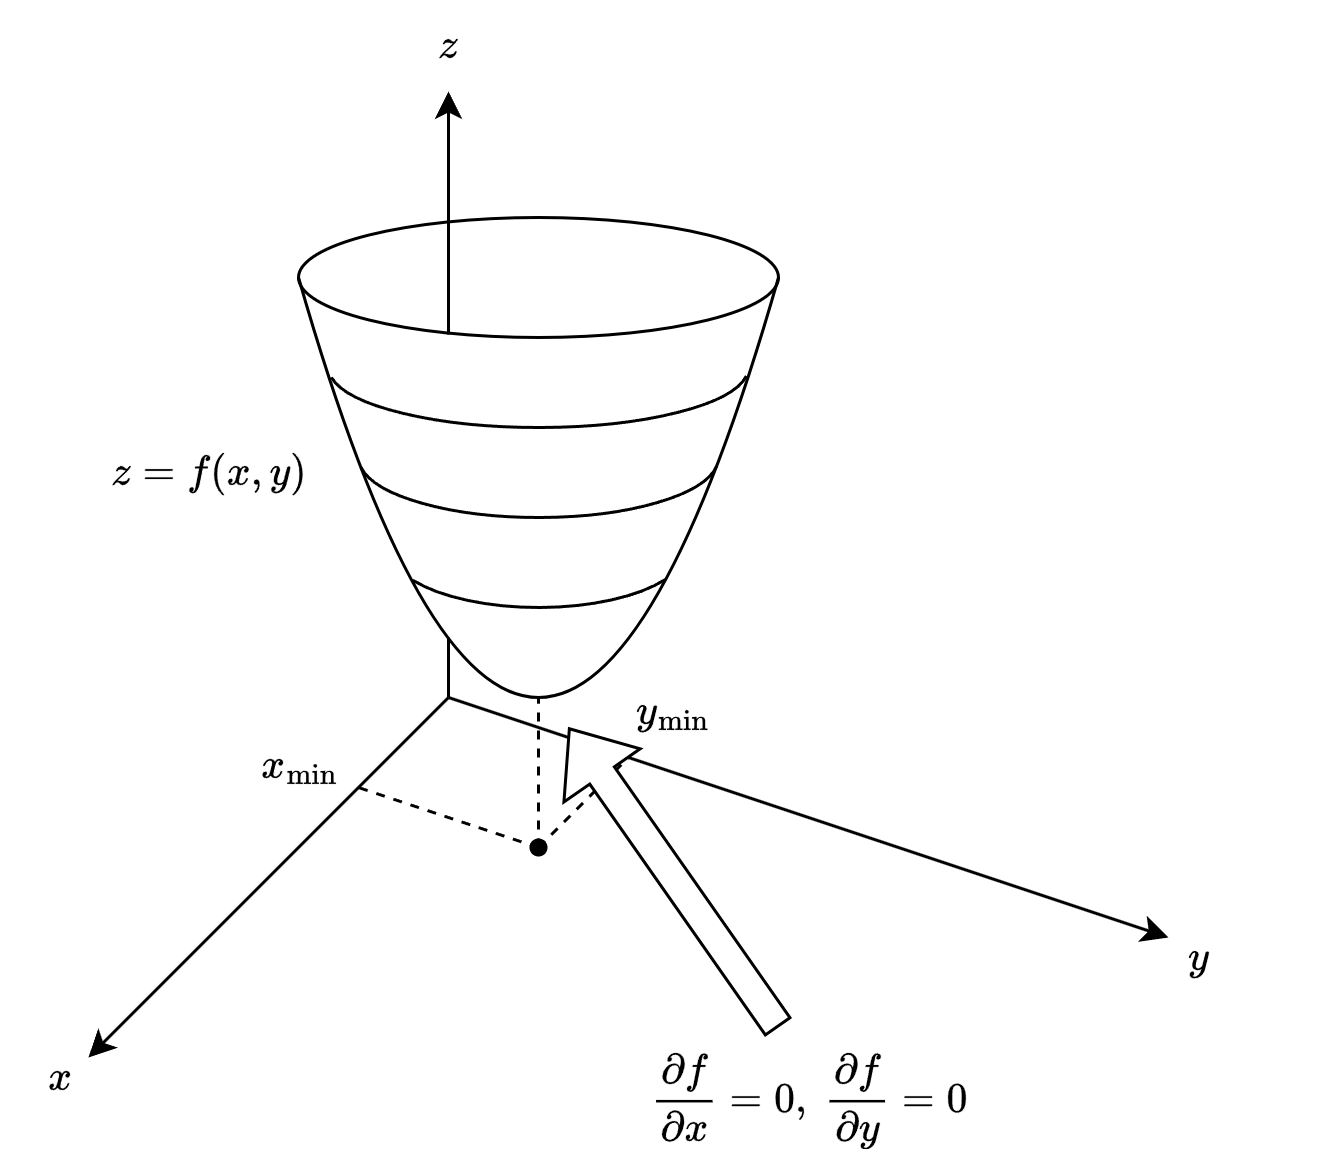
\includegraphics[width=0.6\linewidth]{img/image-of-the-parameters-that-take-the-minimum-value-of-multivariable-function}
		\end{figure}
	\end{frame}
	\begin{frame}{斜面を転がるボールのイメージ}
		\begin{figure}
			\centering
			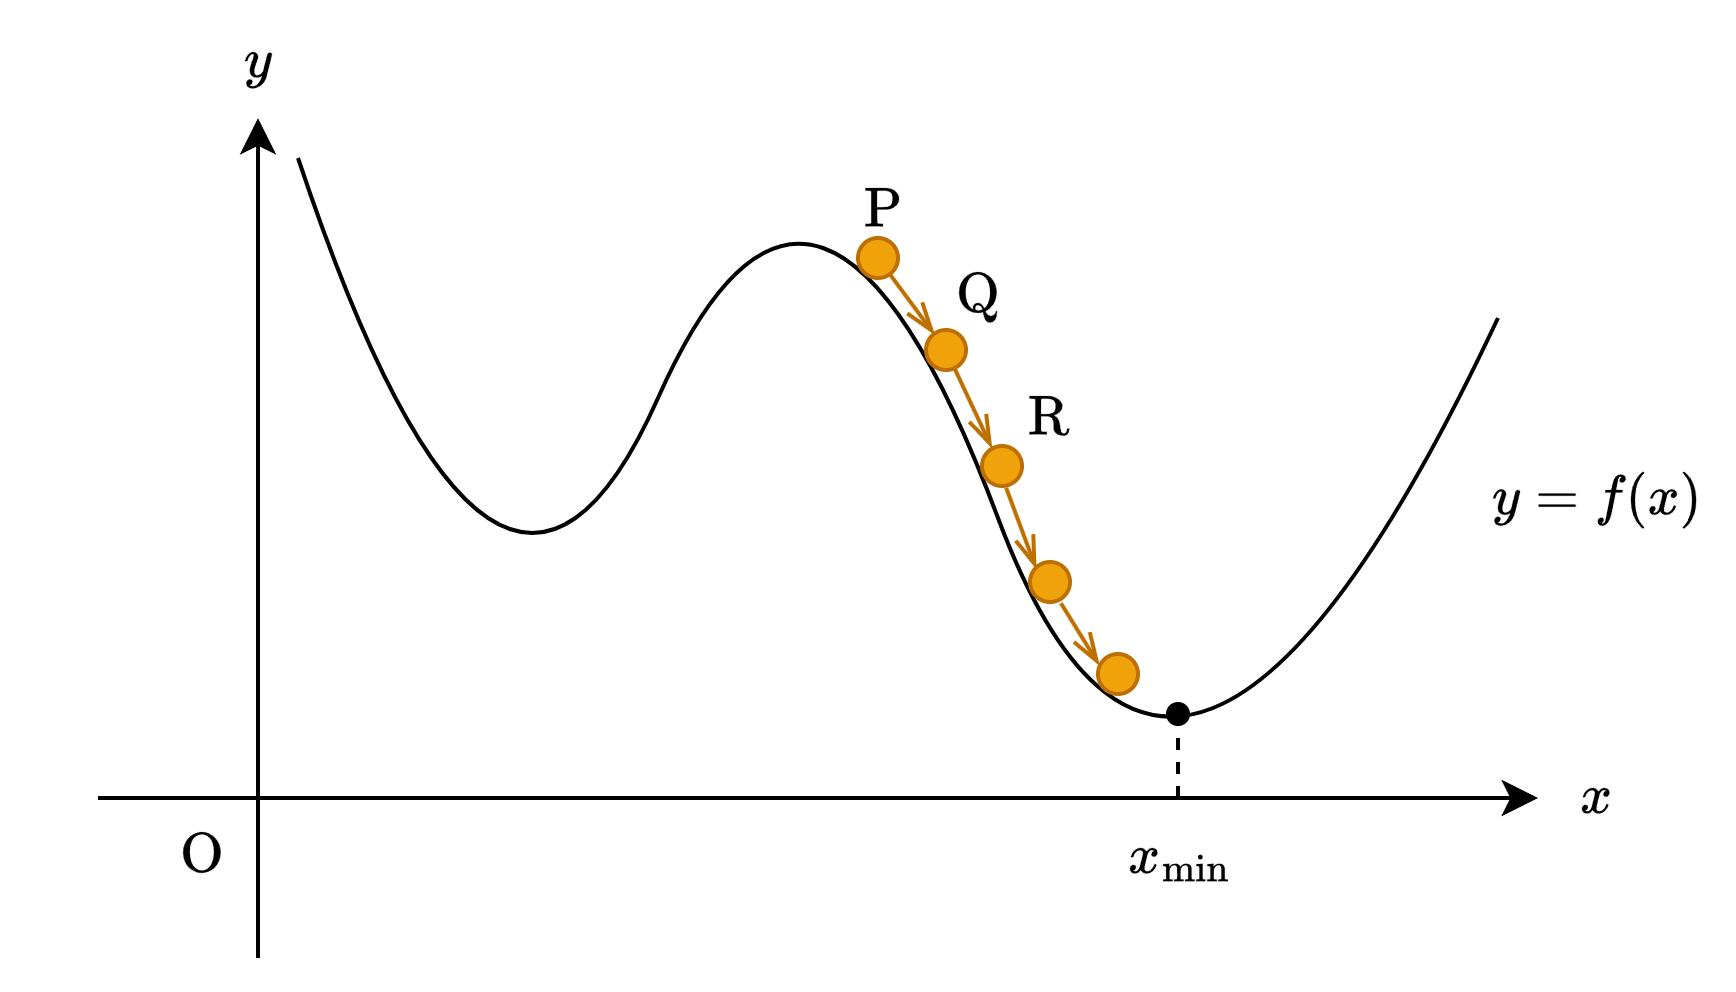
\includegraphics[width=0.7\linewidth]{img/image-of-a-ball-rolling-down-a-slope}
		\end{figure}
	\end{frame}
	\begin{frame}{斜面を転がるボール(多変数関数 ver.)}
		\begin{figure}
			\centering
			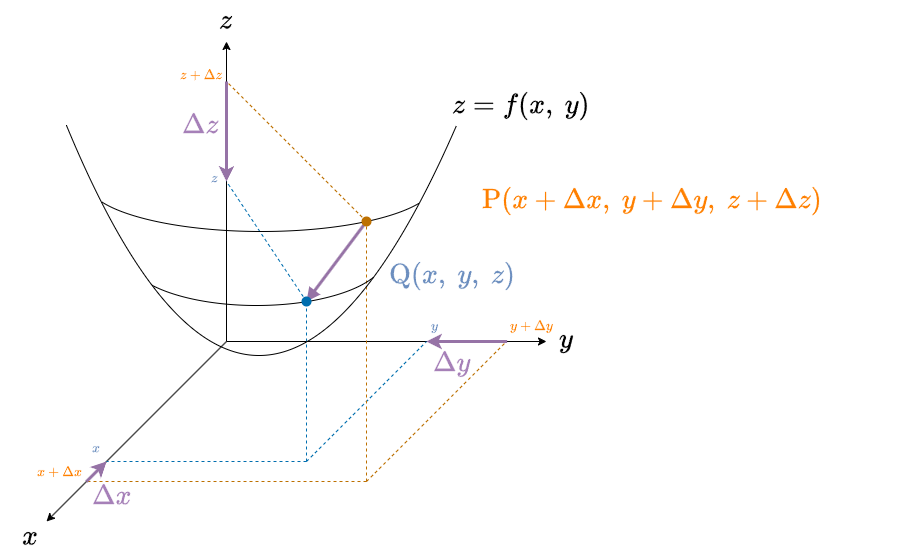
\includegraphics[width=0.7\linewidth]{img/change-in-value-of-a-multivariable-function}
		\end{figure}
		\begin{itemize}
			\item $ \Delta x,\ \Delta y $は具体的にどう決める?
		\end{itemize}
	\end{frame}
	\begin{frame}{勾配降下法の基本式}
		\begin{screen}
			$ \begin{bmatrix}
				\Delta x\\ \Delta y
			\end{bmatrix} = -\eta \begin{bmatrix}
				\dfrac{\partial z}{\partial x}\vspace{1em}\\ \dfrac{\partial z}{\partial y}
			\end{bmatrix} $($ \eta $:正の小さな定数)
		\end{screen}
	\end{frame}


	\begin{frame}{【参考】ギリシャ文字一覧}
		\begin{table}[]
			\begin{tabular}{ll|ll}
				\toprule
				文字         & 名称    & 文字         & 名称    \\
				\midrule
				$\alpha$   & アルファ  & $\nu$      & ニュー   \\
				$\beta$    & ベータ   & $\xi$      & グザイ   \\
				$\gamma$   & ガンマ   & $o$        & オミクロン \\
				$\delta$   & デルタ   & $\pi$      & パイ    \\
				$\epsilon$ & イプシロン & $\rho$     & ロー    \\
				$\zeta$    & ゼータ   & $\sigma$   & シグマ   \\
				$\eta$     & イータ   & $\tau$     & タウ    \\
				$\theta$   & シータ   & $\upsilon$ & ウプシロン \\
				$\iota$     & イオタ   & $\phi$     & ファイ   \\
				$\kappa$   & カッパ   & $\chi$     & カイ    \\
				$\lambda$  & ラムダ   & $\psi$     & プサイ   \\
				$\mu$      & ミュー   & $\omega$   & オメガ  \\
				\bottomrule
			\end{tabular}
		\end{table}
	\end{frame}
\end{document}
